\chapter{はじめに}
\label{chapter: introduction}

\section{問題設定}
\label{section: problemDefinition}
所与の領域を一人または複数の巡査が動き回り,
その領域内の指定された場所を十分な頻度で訪れることを
警邏(patrolling)という\cite{
  40021287065,
  dumitrescu2014fence,
  coene2011charlemagne,
  czyzowicz2011boundary,
  Dumitrescu:2014:CGC:2636805.2636822}.

本論文では,与えられた距離空間$U$内を巡査$m$人が速さ$1$以下で動きまわることにより,
有限集合$V \subseteq U$に属する点を十分な頻度で訪れるという目標を考える.
距離空間$U$といっても,
$V$の点どうしを結ぶ最短路以外を歩むことは無駄であるから,
$V$を頂点集合として辺に長さのついたグラフを考え,
$U$はその頂点および辺上の点のみからなるとしてよい.
このような空間と点集合の組$(U, V)$を\defword{地図}と呼ぶ.

地図$(U, V)$における
巡査$i \in \{1, \ldots, m\}$の\defword{運行}$a _i \colon \Rset \to U$とは,
各時刻$t \in \Rset$における位置$a _i (t) \in U$を定める函数であって,
移動の速さが$1$以下であるもの,すなわち
任意の時刻$s, t \in \Rset$に対し$a _i (s)$と$a _i (t)$の距離が$\abs{s - t}$を超えないものをいう.
巡査$m$人による\defword{運行}とは,
全巡査の運行を定めた組$(a _1, \dots, a _m)$をいう.
$V$の各点には\defword{利得}および\defword{{\maxIdletime}}と呼ばれる正整数が定まっている.
点$v \in V$の{\maxIdletime}が$q$であるとき,
巡査達が運行$(a _1, \dots, a _m)$で点$v$を\defword{警邏}するとは,
長さ$q$のどの時間にも
いずれかの巡査が$v$を少なくとも一度は訪れる
(任意の時刻$t \in \Rset$に対して
巡査$i$と時刻$\tau \in [t, t + q)$が存在し$a _i (\tau) = v$)
ことをいう.
巡査達が運行$A$により集合$W \subseteq V$に属するすべての点を警邏するとき,
巡査達は$A$により$W$を\defword{警邏}するという.

\begin{patrollingProblem}
  巡査の人数$m \in \Nset$と地図$(U, V)$および
  $V$の各点の利得と{\maxIdletime}が与えられる.
  $m$人の巡査により全点を警邏できる$V$の部分集合のうち
  利得の和が最大となるものを求めよ.
\end{patrollingProblem}

また,全点を警邏できるか否かを判定する問題を\defword{\PP}と呼ぶ.

一つの点を複数の巡査の訪問により警邏し得ることに注意されたい.
例えば図\ref{figure: cooperative}左はそのような運行の例である.
\begin{figure}
  \centering
  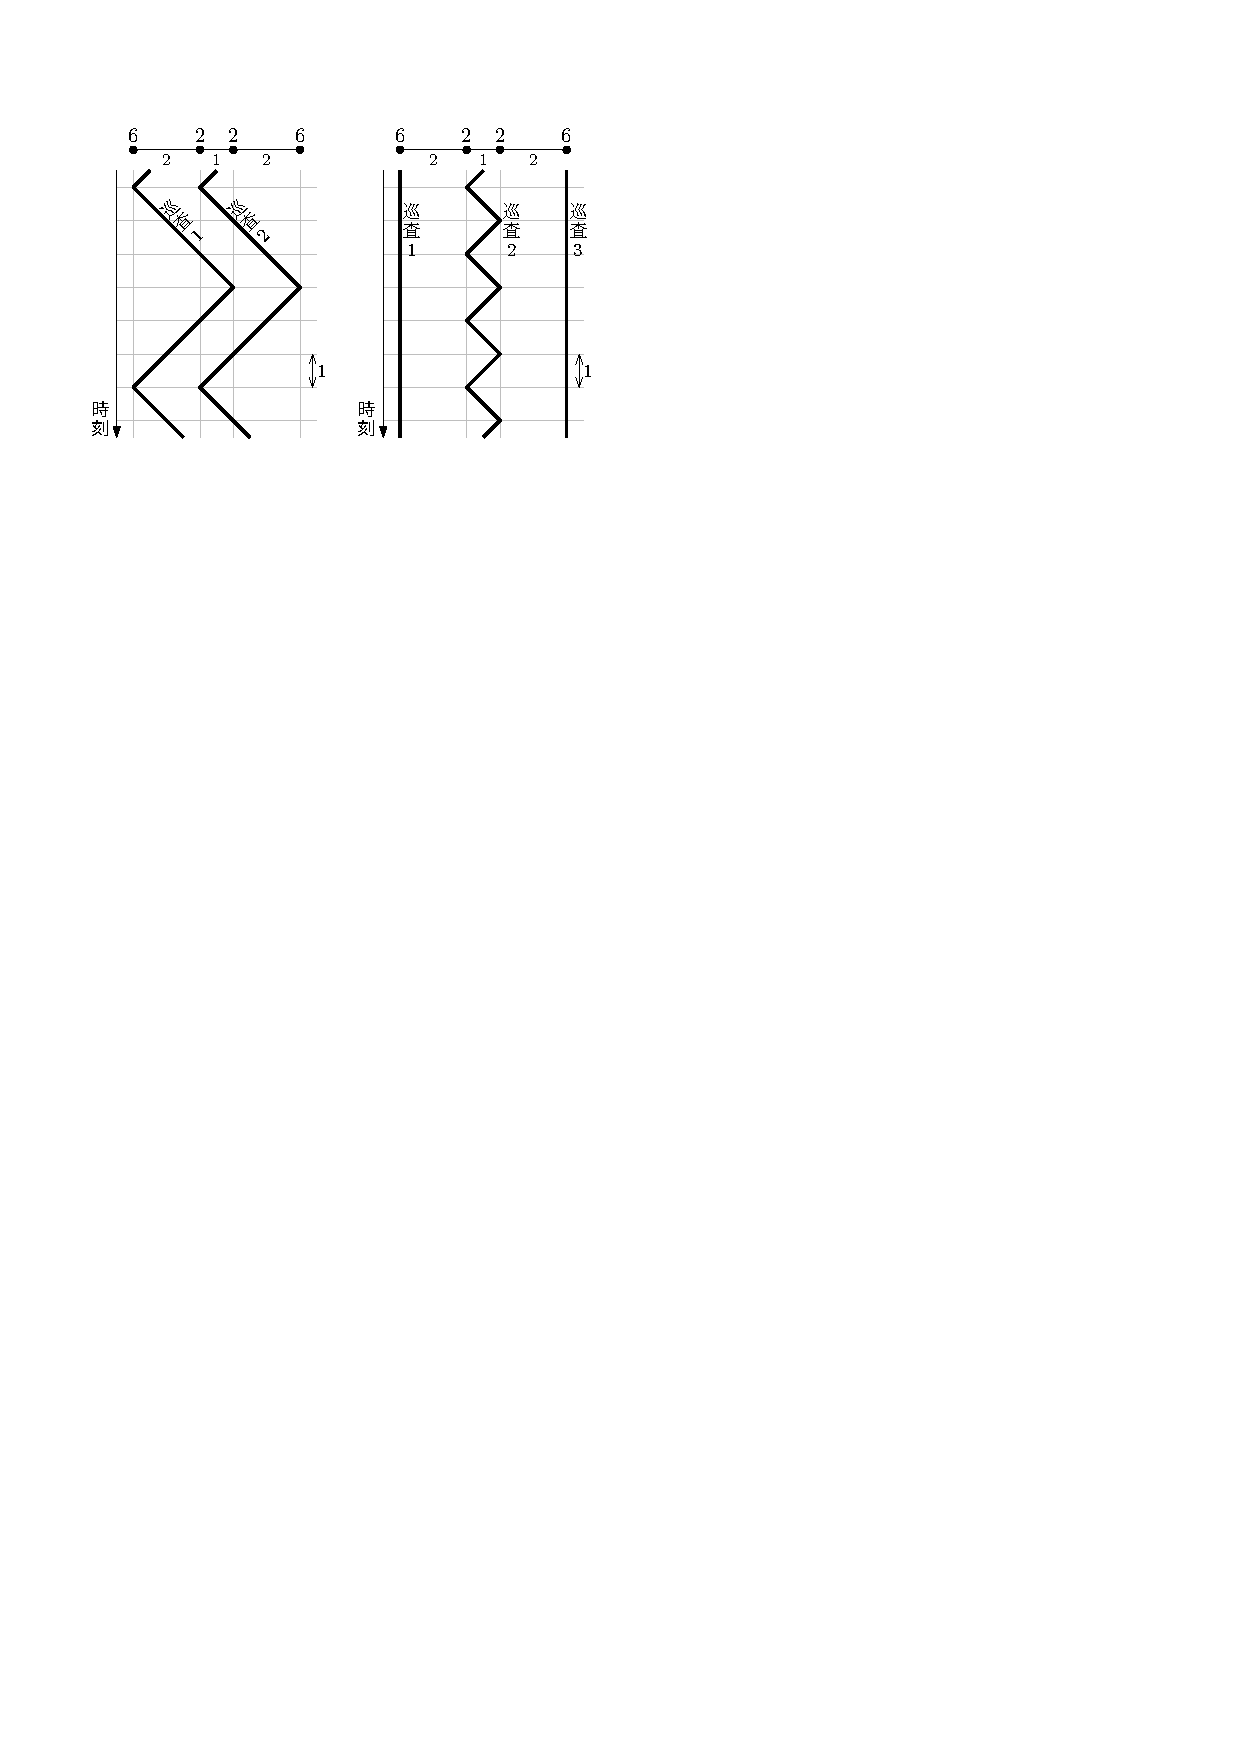
\includegraphics[scale=1.0]{\figdir/cooperative.pdf}
  \caption{図の上部に描かれた地図において,四つの点すべてを警邏する二つの運行.
    点と辺に書かれた数は,それぞれ{\maxIdletime}と距離である.
    左図の運行では二人の巡査が協力して中央の二点を警邏している.
    これを禁じ,各点をいずれかの巡査が単独で警邏することを求めると,
    右図のように三人の巡査を要する.}
  \label{figure: cooperative}
\end{figure}
Coeneら\cite{coene2011charlemagne}は似た問題を扱っているが,
このような協力を許さず,
図\ref{figure: cooperative}右のように
各点$v \in W$に対して一人の巡査がおり,
その巡査のみの運行が$v$を警邏することを要求している.
対比のため本論文ではこの問題を\defword{\independentPP}と呼ぶことにする
(\cite{coene2011charlemagne}ではMPLPPと称している).
Coeneら\cite{coene2011charlemagne}の諸結果においては
この限定が,
多項式時間算法の設計にも困難性の証明にも使われた.
この限定を外したときの様子を調べるのが本論文の目的である.

{\PP}は,巡査が一人かつ
全点の{\maxIdletime}が等しい場合に限っても,
ハミルトン路問題からの帰着により
NP困難である\cite[Theorem~8]{coene2011charlemagne}.
そこで本論文では入力される地図$(U, V)$を次のそれぞれの形状に限定する
(図\ref{figure: graph_classes}).
%
\begin{figure}
  \centering
  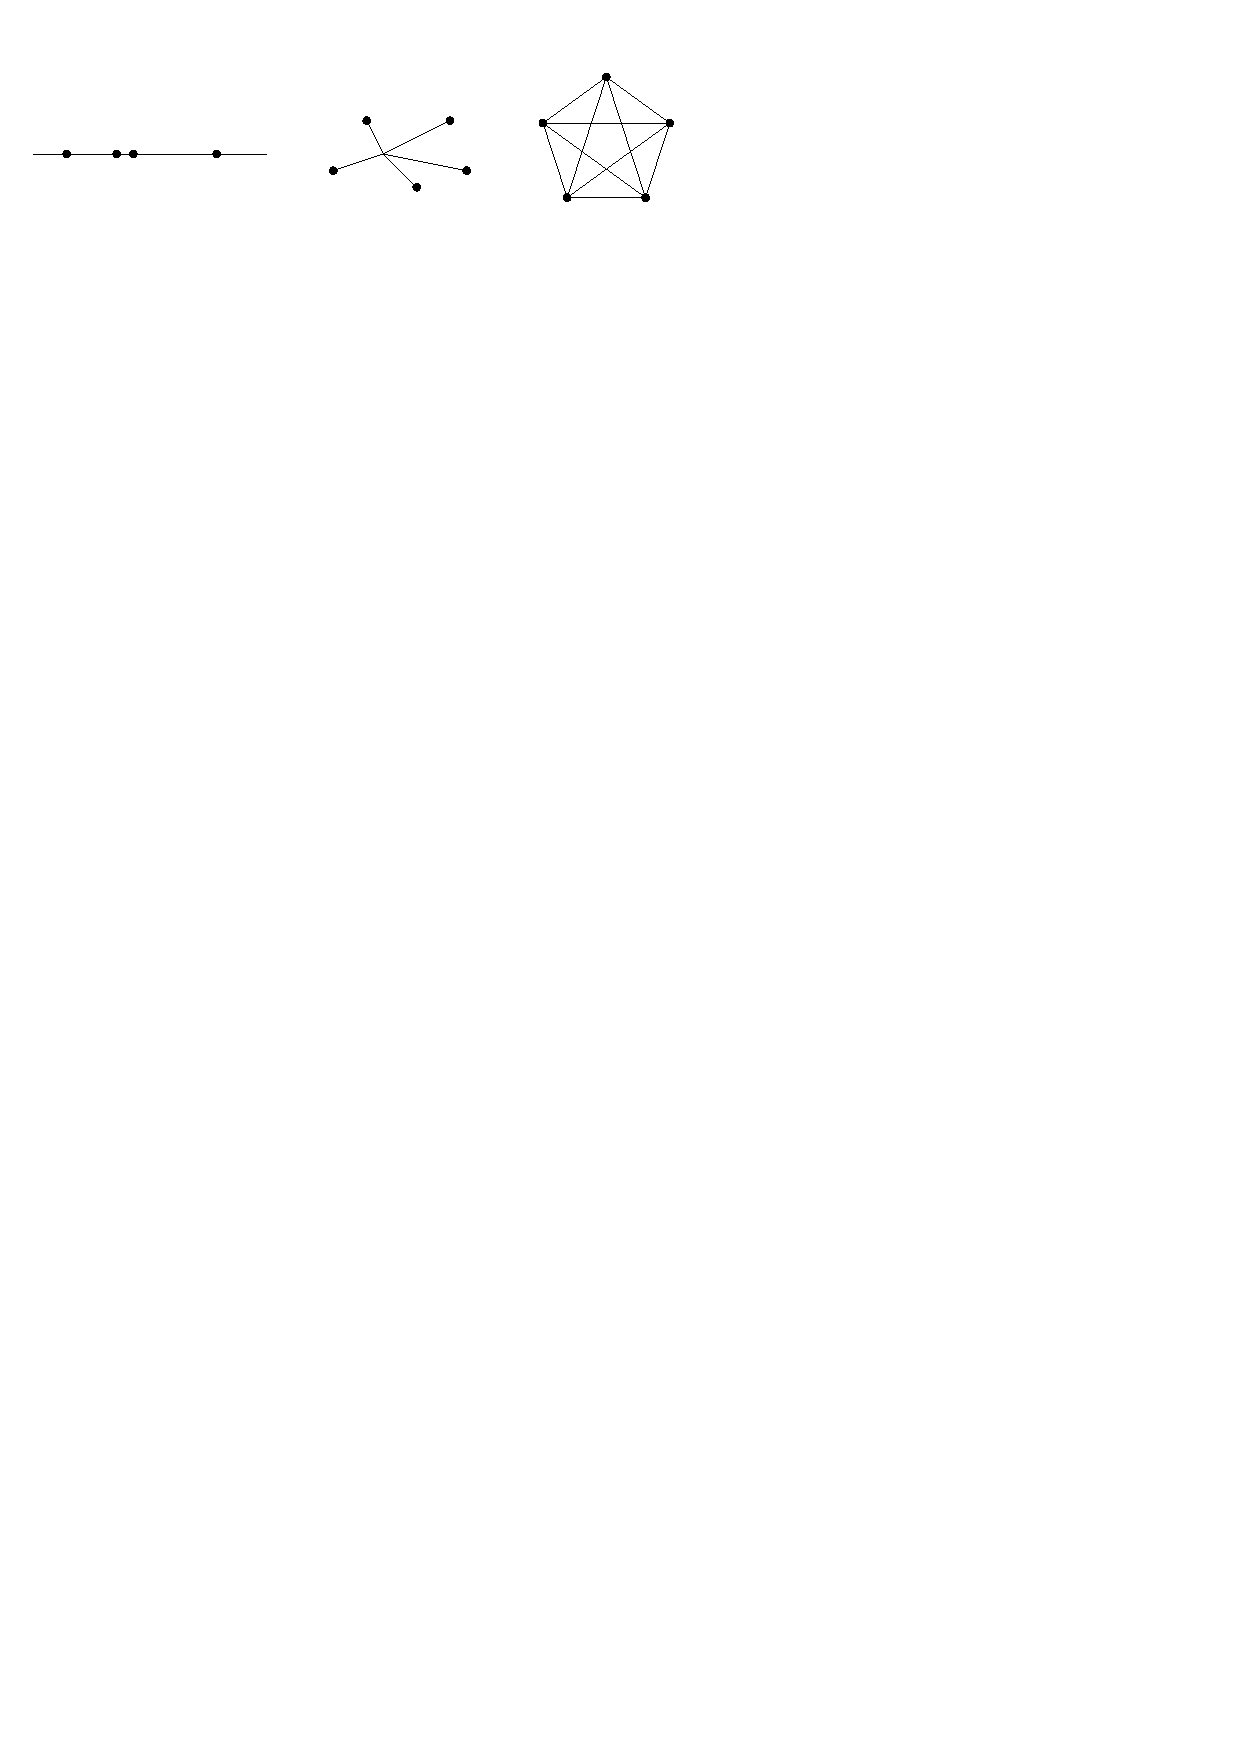
\includegraphics[scale=1.0]{\figdir/graph_classes.pdf}
  \caption{本論文では
    {\graphLine}(左),{\graphStar}(中),{\graphUnit}(右,但し各辺の長さが等しい)を扱う.
    {\graphStar}は葉のみを警邏の対象とする(中心は移動の途中で使うのみであり,
    {\maxIdletime}は定められていない).}
  \label{figure: graph_classes}
\end{figure}
%
\begin{description}
  \item[{\graphLine}]
    $U$は直線である.
  \item[{\graphStar}]
    $U$は\defword{中心}と呼ばれる一点を
    各点$v \in V$へ結ぶ辺のみからなる.
  \item[{\graphUnit}]
    $V$の各二点間に辺があり,その長さはすべて等しい.
\end{description}
%
{\graphLine}では$V$の全点の外側の領域,
{\graphStar}では中心という特別な点を$U$は含んでいるが,
{\PPProfit}の入力の地図には$V$と$V$の点どうしの距離の情報があればよく,
{\graphStar}も$V$上の完全グラフに適切に辺の長さを定めたものとみることができるので
(図\ref{figure: stars}),
冒頭で述べたように$V$上のグラフとして与えられるとして差し支えない.
% このうち{\graphLine}や{\graphStar}では,
% $U$は警邏すべき対象である$V$の点どうしを結ぶ最短路以外の部分を含んでいるが,
% {\graphLine}では$V$の全点の外側にある部分を歩むことは無駄であるし,
% {\graphStar}も$V$上の完全グラフに適切に辺の長さを定めたものとみることができるので
% (図\ref{figure: stars}),
\begin{figure}
  \centering
  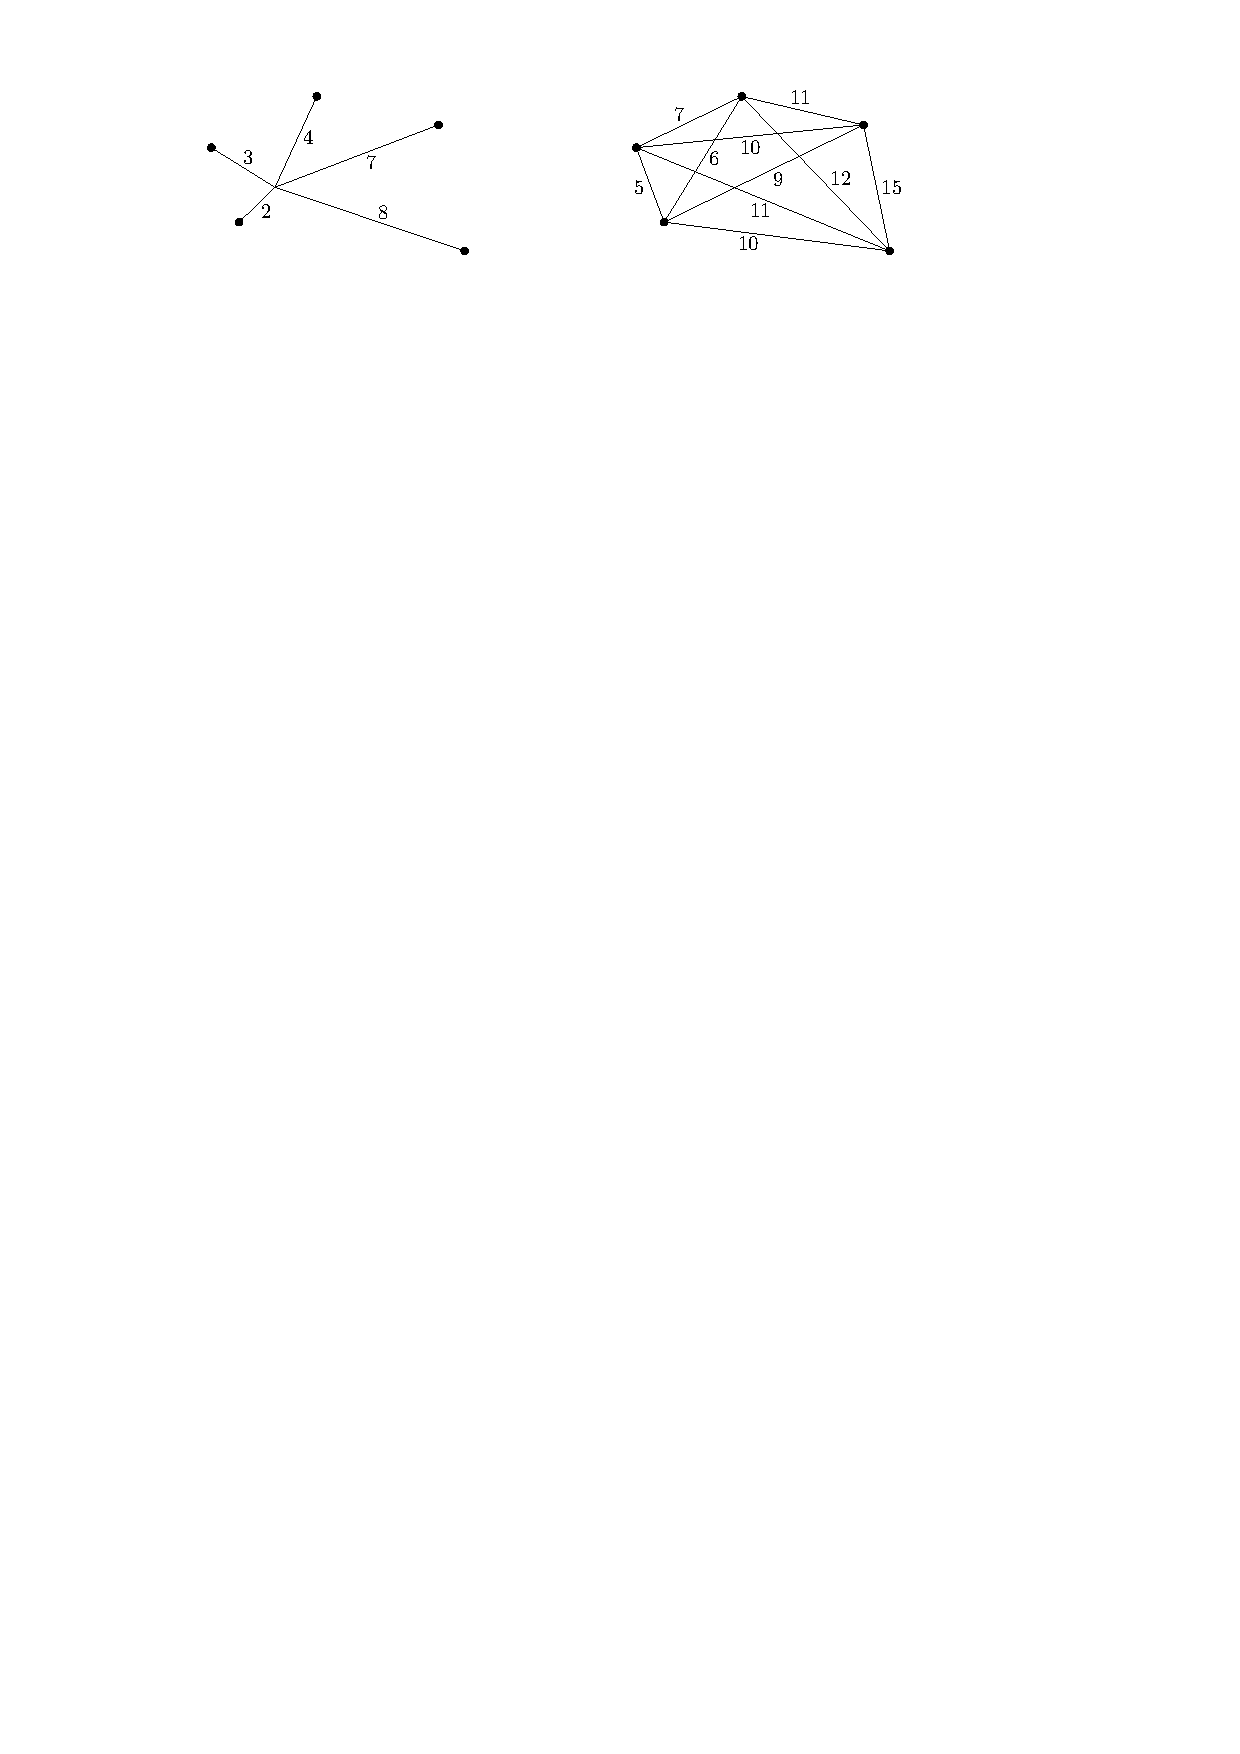
\includegraphics[scale=1.0]{\figdir/stars.pdf}
  \caption{左図の{\graphStar}は,各二点間に右図のような距離を定める.}
  \label{figure: stars}
\end{figure}
% 地図は冒頭で述べたように$V$上のグラフとして与えられると考えて差支えない.
なお,このように考えると各辺の長さが$d$の{\graphUnit}は,
中心から各点への距離が$d/2$の{\graphStar}と同じであるから,
{\graphUnit}は{\graphStar}の特殊な場合である.

{\PPProfit}についての我々の結果を
Coeneらの{\independentPP}についての結果との比較も含めて
地図の形ごとにまとめると次のようになる.
それぞれ\ref{chapter: line},\ref{chapter: star},\ref{chapter: unit}章で述べる.
\begin{itemize}
\item 
  {\graphLine}の
  {\independentPP}は動的計画法により多項式時間で解けることが
  示されていた\cite[Theorem~11]{coene2011charlemagne}.
  本論文では複数人が一点を警邏することを認めた{\PPProfit}について,
  全点の{\maxIdletime}が等しい場合には多項式時間で解けることを示す
  (定理\ref{theo:LineUnaryIdletimePolyTimeSolvable}).
\item
  {\graphStar}については,
  全点の利得と{\maxIdletime}が等しい場合に限っても,
  {\independentPP}はNP困難であることが示されていた\cite[Theorem~10]{coene2011charlemagne}.
  本論文では,この場合の{\PPProfit}は多項式時間で解けるという興味深い結果を得る
  (定理\ref{theo:StarUnaryProfitAndIdletime}).
  なお利得または{\maxIdletime}を一般にすると,
  巡査が一人であっても(したがって独立かどうかによらず)
  NP困難であることがわかっている\cite[Theorems 5 and 6]{coene2011charlemagne}.
\item 
  {\graphUnit}については,
  本論文では全点の{\maxIdletime}が等しい場合は{\PPProfit}が多項式時間で解けることを示す
  (定理\ref{theo:UnitUnaryIdletime}).
  地図が{\graphStar}の場合は
  巡査が一人で全点の{\maxIdletime}が等しくても利得が一般だとNP困難になる
  \cite[Theorem~5]{coene2011charlemagne}ので,
  {\graphUnit}は{\graphStar}よりも簡単に解ける形状と言える.
\end{itemize}

{\graphLine}や{\graphUnit}については,
全点の{\maxIdletime}が等しい場合には上述のように
多項式時間アルゴリズムを見つけることができたが,
{\maxIdletime}が一般の場合にはそれができなかった.
{\graphStar}の{\PPProfit}は上述の通りNP困難なので\cite[Theorems 5 and 6]{coene2011charlemagne},
{\graphLine}や{\graphUnit}についても
NP困難ではないかと予想したが,これも示すことができなかった.
これらの未解決な場合については,
警邏ではなく定時訪問を目指す次のような問題を考えた.

\begin{timeSpecifiedPatrollingProblem}
  巡査の人数$m \in \Nset$と地図$(U, V)$および
  $V$の各点の利得と{\exactTime}が与えられる.
  % $m$人の巡査の運行により$V$の全点を定時訪問できるか判定せよ.
  $m$人の巡査の運行により全点を定時訪問できる$V$の部分集合のうち
  利得の和が最大となるものを求めよ.
  ただし,
  点$v \in V$の{\exactTime}が
  $(q, r)\ (q \in \Nset, r \in \{ 0, 1, \ldots, q - 1 \})$%
  であるとき,
  巡査達が運行$A = (a _1, \ldots, a _m)$で点$v$を\defword{定時訪問}するとは,
  任意の時刻$t := q k + r\ (k \in \Zset)$に対し
  巡査$i$が存在し$a _i (t) = v$であることをいう.
\end{timeSpecifiedPatrollingProblem}

また,全点を定時訪問できるか否かを判定する問題を\defword{\timeSpecifiedPP}と呼ぶ.

{\graphLine}については{\timeSpecifiedPP}を解く貪欲アルゴリズムを
\ref{section:LineArbitraryIdletime}節で示す.
{\graphUnit}については{\timeSpecifiedPPProfit}がNP困難であることを示す(定理\ref{theo:UnitExacIdletimeNPhard}).


本論文は,
2017年電子情報通信学会総合大会\cite{ieice}%
及び
Japan Conference on Discrete and Computational Geometry, Graphs, and Games 2017\cite{jcdcggg}%
で発表した内容を含む.
